\chapter{Integrali multipli}
Il capitolo che segue espone la teoria dell'integrazione di funzioni di $n$ variabili. La trattazione affronterà in prima istanza il tema della misura secondo Peano-Jordan. Dopodiché si passerà al caso degli integrali doppi con funzioni di $n=2$ variabili. Verranno mostrati in seguito i metodi di integrazione di funzioni in $n=3$ variabili, per concludere con gli integrali impropri.
\section{Misura di Peano-Jordan}
\begin{definition} \label{Def: Rettangolo}
Sia $I=\left[a_1, b_1\right) \times \left[a_2, b_2 \right) \times \dots \times \left[a_n, b_n \right)$ con $a_i < b_i$. Allora, tale intervallo è definito \textbf{rettangolo} superiormente semiaperto di $\mathbb{R}^n$.\\
Inoltre, si definisce \textbf{misura elementare} di $I$ il volume di tale rettangolo, cioè:
\begin{equation}
    m(I)=\left(b_1-a_1\right)\left(b_2-a_2\right)\dots\left(b_n-a_n\right)
\end{equation}
\end{definition}
\begin{oss}
    Se $I$ è vuoto, allora si pone per convenzione $m(I)=0$.
\end{oss}
\begin{oss}
    La scelta di intervalli semiaperti superiormente permette di poter creare partizioni senza problemi di sovrapposizione.
\end{oss}
\begin{definition} \label{Def: Plurirettangolo}
    Si dice \textbf{plurirettangolo} superiormente semiaperto di $\mathbb{R}^n$ un insieme $P$ dato dall'unione finita di rettangoli superiormente semiaperti a 2 a 2 disgiunti, cioè
    \begin{equation}
        P= \bigsqcup_{j=1}^{H \in \mathbb{N}} I_j \qquad I_j \cap I_l = \emptyset\ \text{se}\ j\neq l
    \end{equation}
\end{definition}
\begin{definition} \label{Def: Misura di un plurirettangolo}
Sia $\mathcal{P}= \left\{\text{insieme dei plurirettangoli}\right\}$. Allora si dice \textbf{misura di un plurirettangolo} $P=\bigsqcup\limits_{j=1}^{H} \in \mathcal{P}$ la quantità
\begin{equation}
    m(P)= \sum_{j=1}^{H}{m(I_j)}
\end{equation}
\end{definition}
\begin{oss}
    Si osservi che la scelta di una partizione per $P$ è ininfluente ai fini del calcolo della misura di un plurirettangolo.
\end{oss}
Queste definizioni, permettono di sviluppare una funzione $m: \mathcal{P} \to \mathbb{R}^+$ che goda delle seguenti proprietà $ \forall\ P_1, P_2\in \mathcal{P}$:
\begin{itemize}
    \item $m$ è \textbf{subadditiva}: $m(P_1 \cup P_2) \leq m(P_1)+m(P_2)$
    \item $m$ è \textbf{additiva}: $m(P_1 \cup P_2)=m(P_1)+m(P_2)$ se $P_1 \cap P_2 = \emptyset$
    \item $m$ è \textbf{crescente}: se $P_1 \subseteq P_2$ allora $m(P_1) \leq m(P_2)$
\end{itemize}
\begin{definition} \label{Def: Misura interna, misura esterna}
Sia $E \subseteq \mathbb{R}^n$. Allora, si definisce \textbf{misura esterna} di E la quantità 
\begin{equation}
    \overline{m}(E) := \inf\left\{m(P) \mid P \in \mathcal{P}, E \subseteq \mathcal{P} \right\}
\end{equation}
Analogamente, si definisce \textbf{misura interna} di E la quantità
\begin{equation}
    \underline{m}(E) := \sup\left\{m(P) \mid P \in \mathcal{P}, E \subseteq P\right\}
\end{equation}
\end{definition}
\begin{proposition}
    Sia $E \subseteq \mathbb{R}^n$ limitato. Allora $\underline{m}(E) \leq \overline{m}(E)$
\end{proposition}
\begin{definition} \label{Def: Insieme misurabile}
    Si dice che $E \subseteq \mathbb{R}^n$ è \textbf{misurabile} secondo Peano-Jordan se
    \begin{equation}
        \underline{m}(E)=\overline{m}(E)
    \end{equation}
    In tal caso allora
    \begin{equation}
        m(E) := \underline{m}(E)=\overline{m}(E)
    \end{equation}
    e si indica con $\mathcal{M}$ l'\textbf{insieme degli $\mathbf{E}$} limitati e \textbf{misurabili} di $\mathbb{R}^n$
\end{definition}
\begin{oss}
    Una notazione alternativa di $m(E)$ è $m_n(E)$
\end{oss}
\begin{oss}
    Si noti che $\mathcal{M} \subsetneq \mathcal{P}(\mathbb{R}^n)$
\end{oss}
\begin{example}
    A sostegno di quest'ultima osservazione si proponga un insieme non misurabile di $\mathbb{R}^n$
    \begin{equation*}
        \Tilde{E}=\left( \left[0,1\right] \cap \mathbb{Q}^2\right)
    \end{equation*}
    Infatti, volendo coprire di plurirettangoli tale insieme, si ha che:
    \begin{align*}
        &\overline{m}(\Tilde{E})=1=(1-0)\times(1-0)\\
        &\underline{m}(\Tilde{E})=0
    \end{align*}
    Pertanto $\Tilde{E}$ non è misurabile secondo Peano-Jordan.
\end{example}
D'altro canto, si elenchino ora tipi di insiemi che siano Peano-Jordan misurabili.
\begin{example}
    Il caso banale è il plurirettangolo P. Infatti:
    \begin{equation*}
    m(P)=m(\mathring{P})=m(\overline{P})       
    \end{equation*}
\end{example}
\begin{example}
    Un \textit{dominio semplice}, cioè un dominio compreso tra i grafici di funzioni continue su $\left[a,b\right]$ limitate, è P.J. misurabile.
    
    In $\mathbb{R}^2$ si possono avere domini semplici della forma:
    \begin{equation*}
            D= \left\{ (x, y) \in \mathbb{R}^2 \mid a \leq x \leq b ,\ f(x)\leq y \leq g(x) \right\}\        
    \end{equation*}
    detti \textit{y-semplici} o \textit{normali rispetto all'asse x}. Oppure
    \begin{equation*}
        E= \left\{(x, y) \in \mathbb{R}^2\mid c \leq y \leq d,\ h(y) \leq x \leq l(y)\right\}
    \end{equation*}
    detti \textit{x-semplici} o \textit{normali rispetto all'asse y}.
    \vspace*{6pt}                       
    
    In $\mathbb{R}^3$ esempi di domini semplici possono essere:
    \begin{equation*}
        \mathcal{D}=\left\{(x,y,z) \in \mathbb{R}^3 \mid (x,y) \in D \subseteq \mathbb{R}^2,\ \alpha(x, y) \leq \beta(x,y) \right\}
    \end{equation*}
    con $D$ normale rispetto ad almeno un asse e detto \textit{z-semplice} o \textit{normale rispetto al piano xy} o, ancora \textit{rappresentabile per fili}. Oppure, 
    \begin{equation*}
        \mathcal{E}=\left\{(x,y,z) \in \mathbb{R}^3 \mid c_1 \leq z \leq c_2,\ (x,y) \in D_z\subseteq \mathbb{R}^2\right\}
    \end{equation*}
    con $D_z$ dominio normale e detto \textit{xy semplice} o \textit{normale rispetto all'asse $z$} o \textit{rappresentabile per strati}.
\end{example}
    \begin{oss}
        Si possono ottenere altri domini normali di $\mathbb{R}^3$ invertendo gli assi.
    \end{oss}
    \begin{oss}
        Se $D$ è un dominio normale rispetto a $x$, si ha che
        \begin{equation}
            m(D)= \int_a^b(g(x)-f(x))dx
        \end{equation}
        Lo stesso discorso vale poi per domini semplici di $\mathbb{R}^3$. Infatti
        \begin{equation}
            \begin{aligned}
                &m(\mathcal{D})=\iint_D(\beta(x,y)-\alpha(x,y))dxdy\\
                &m(\mathcal{E})=\int_{c_1}^{c_2}(m_z(D_z))dz
            \end{aligned}
        \end{equation}
    \end{oss}
    \subsection{Proprietà della misura di Peano-Jordan}
    Siano $A, B \in \mathcal{M}$. Allora, si può osservare che l'unione, l'intersezione e la differenza di insiemi misurabili è misurabile.
    \begin{equation}
        A \cup B,\ A \cap B,\ A \setminus B \in \mathcal{M}
    \end{equation}
    Rispetto a ciò, per \textbf{subadditività}, la misura dell'unione vale:
    \begin{equation}
        m(A \cup B) = m(A)+ m(B)- m(A \cap B)
    \end{equation}
    e, in particolare, se l'intersezione dei due insiemi è vuota, vale l'\textbf{additività finita}, cioè:
    \begin{equation}
        m(A \cup B) = m(A)+ m(B)
    \end{equation}
    Per quanto riguarda la misura della differenza dei due insiemi si nota che 
    \begin{equation}
        m(A \setminus B)= m(A)-m(A \cap B)
    \end{equation}
    e, nello specifico, se $B \subseteq A$,
    \begin{equation}
        m(B) \leq m(A)
    \end{equation}
    per \textbf{monotonia}.\\
    Infine $E \subseteq \mathbb{R}^n$ limitato è misurabile se e solo se la sua frontiera $\partial E$ è misurabile ed ha misura nulla.
\section{Introduzione agli integrali multipli}
Si descriva ora il processo di costruzione degli integrali in più variabili tramite l'utilizzo delle somme superiori e inferiori di Riemann.

D'ora in avanti si considerino $A \subseteq \mathbb{R}^n$ aperto con $A \in \mathcal{M}$ e $f:A \to \mathbb{R}$ limitata. Si prenda poi poi $P=\left\{ A_i \right\}_{i=1}^{N}$ una partizione finita di $A$ di insiemi misurabili secondo Peano-Jordan, cioè tale che
    \begin{equation}
    A= \bigsqcup A_i \qquad A_i \in \mathcal{M}\ \forall\ i
    \end{equation}
\begin{definition} \label{Def: Somme di Riemann}
Con le premesse sopra, si dicono \textbf{somme inferiori} di $f$ associate a $P$
\begin{equation}
    s(P)= \sum\limits_{i=1}^{N}\inf_{A_i} f\ m(A_i)
\end{equation}
e si dicono analogamente \textbf{somme superiori} di $f$ associate a $P$
\begin{equation}
    S(P)= \sum\limits_{i=1}^{N}\sup_{A_i}f\ m(A_i)
\end{equation}
È evidente che $s(P) \leq S(P)\ \forall P$.
Perciò detto $\Pi$ insieme delle partizioni finite e misurabili di $A$ si ha che
\begin{equation}
    \sup_{P \in \Pi(A)} s(P) \leq \inf_{P \in \Pi(A)} S(P)
\end{equation}
\end{definition}
\begin{definition} \label{Def: Integrale e integrabilità}
    Sia $f: A \to \mathbb{R}^n \in \mathcal{M}$ limitata. Allora $f$ si dice \textbf{integrabile} secondo Riemann in $A$ se 
    \begin{equation}
        \sup_{P \in \Pi(A)} s(P) = \inf_{P \in \Pi(A)} S(P)= \ell
    \end{equation}
    In tal caso, si definisce l'\textbf{integrale di Riemann} come
    \begin{equation}
        \int_A{f(x_1, \dots, x_n)}dx_1\dots dx_n := \ell
    \end{equation}
\end{definition}
Un importante risultato circa la teoria dell'integrazione è quello ottenuto dal teorema che segue.
\begin{theorem} [Integrabilità delle funzioni continue] \label{Teo: Integrabilità di funzioni continue}
    Sia $f: \overline{A} \to \mathbb{R}$ continua con $A \in \mathcal{M}$, allora $f$ è integrabile su A.
\end{theorem}
\begin{oss}
    Si può notare che $\overline{A}$ è chiuso per la definizione \ref{Def: Insieme chiuso e chiusura}. Inoltre, poiché $A$ è misurabile, per la definizione \ref{Def: Insieme misurabile}, è limitato. Dunque $\overline{A}$ è compatto.
\end{oss}
\begin{example}
    Si faccia ora l'esempio di una funzione limitata ma non integrabile secondo Riemann. Sia $f: [0,1]^2 \to \mathbb{R}$
    \begin{equation*}
    f(x, y)=\begin{cases}
        1 \quad & (x,y) \in [0,1]^2 \cap \mathbb{Q}^2\\
        0 \quad & (x,y) \notin [0,1]^2 \cap \mathbb{Q}^2
    \end{cases}
    \end{equation*}
    In tale funzione si osserva che per qualsiasi partizione vale
    \begin{equation*}
        s(P)=0 \qquad S(P)=1 
    \end{equation*}
    pertanto la funzione non è integrabile secondo Riemann. [Ma lo sarà secondo Lebesgue]
\end{example}
\subsection{Proprietà dell'integrale multiplo}
Sia $D \in \mathcal{M}$ e siano $f, g$ integrabili su $D$.
Allora si può affermare che, per \textbf{linearità}
\begin{equation}
    \int_D{(\lambda f+ \mu g)}= \lambda \int_D{f}+ \mu \int_D g
\end{equation}
Inoltre, se $ f \geq g$ su $D$, vale la \textbf{monotonia}, perciò
\begin{equation}
    \int_D{f} \geq \int_D{g}
\end{equation}
Infine, presa una partizione $P$ di $D$ tale che $D= \bigsqcup\limits_{i=1}^{N} D_j$ con $D_j \in \mathcal{M}$, allora per \textbf{additività} vale
\begin{equation}
    \int_D{f}= \sum\limits_{j=1}^{N}{\int_{D_j}{f}}
\end{equation}
\subsection{Integrali doppi}
Il processo di costruzione dell'integrale doppio è esattamente quello presentato prima, con l'accortezza di considerare $n=2$.\\
All'interno del paragrafo verranno presentate le formule di riduzione degli integrali doppi e le formule di cambiamento di variabili.
\subsubsection{Formule di riduzione}
Si considerino i seguenti domini normali:
    \begin{align}
    &D= \left\{ (x, y) \in \mathbb{R}^2 \mid a \leq x \leq b ,\ f(x)\leq y \leq g(x) \right\}\\
    &E= \left\{(x, y) \in \mathbb{R}^2\mid c \leq y \leq d,\ h(y) \leq x \leq l(y)\right\}
    \end{align}
allora, per ogni $F: D \to \mathbb{R}$ continua vale
\begin{equation} \label{Eq: Formula di riduzione integrali doppi 1}
\iint_{D} F(x,y) dxdy = \int_{a}^{b}\left(\int_{f(x)}^{g(x)}{F(x,y)dy}\right)dx 
\end{equation}
Analogamente, data una generica $G: E \to \mathbb{R}$ continua, si ha che
\begin{equation} \label{Eq: Formula di riduzione integrali doppi 2}
    \iint_{E} G(x,y) dxdy = \int_{c}^{d}\left(\int_{h(y)}^{l(y)}{F(x,y)dx}\right)dy 
\end{equation}
Si osservi che l'integrale di funzioni separate $F(x)G(y)$ in un rettangolo $ \left[a,b \right] \times \left[c,d\right]$ è il prodotto degli integrali, cioè:
\begin{equation}
    \iint_{\left[a,b \right] \times \left[c,d\right]}{F(x)G(y)}\ dxdy = \left(\int_{a}^{b}{F(x)}\ dx \right)\left(\int_{c}^{d}{G(y)}\ dy \right)
\end{equation}
\begin{example}
    Si calcoli il seguente integrale:
    \begin{equation*}
        \iint_{D}{xy}\ dxdy
    \end{equation*}
    dove $D$ è il triangolo di vertici $A=(0,0)$, $B=(1,0)$, $C=(1,1)$.
    \begin{figure}[H]
   \begin{minipage}{0.3\textwidth}
   \centering
   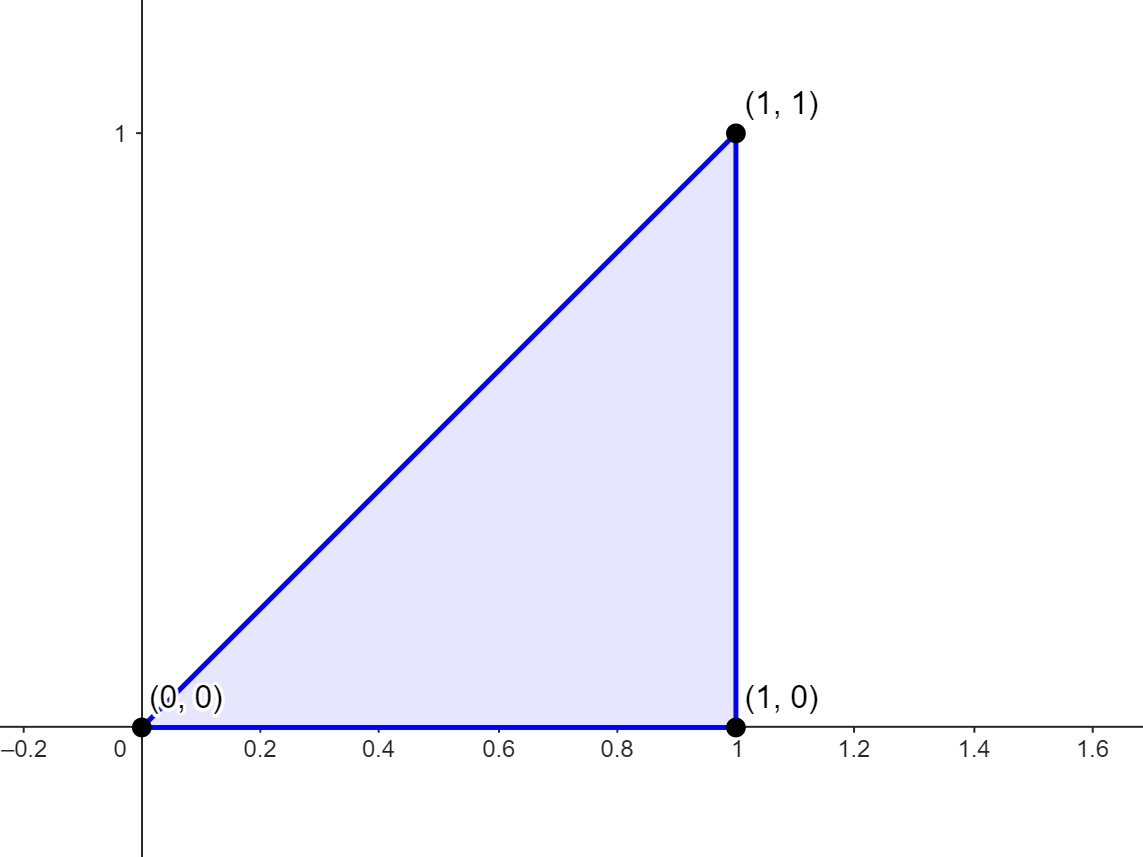
\includegraphics[width=\textwidth]{Capitoli/Capitolo4/Integrale 1.png}
    \end{minipage}
    \hfill
    \begin{minipage}{0.55\textwidth} 
    Tale insieme è un dominio normale sia rispetto all'asse $x$ che rispetto all'asse $y$. Si osservi che il risultato di tale integrale deve essere lo stesso in qualsiasi dei due casi.
    \end{minipage}
    \end{figure}
    Si consideri $D$ normale rispetto all'asse $x$, cioè:
    \begin{equation*}
        D= \left\{(x,y) \mid 0 \leq x \leq 1, 0 \leq y \leq x \right\}
    \end{equation*}
    Allora, applicando le formule di riduzione \eqref{Eq: Formula di riduzione integrali doppi 1}
    \begin{equation*}
    \begin{aligned}
        \iint_D{xy}\ dxdy &= \int_{0}^{1}{\left(\int_{0}^{x}xy\ dy\right)}dx=  \int_{0}^{1}{x\left(\frac{y^2}{2}\Big|_{0}^{x}\right) dx = \int_{0}^{1}\frac{x^3}{2}\ dx} = \frac{1}{8}
    \end{aligned}
    \end{equation*}
    Considerando $D$ normale rispetto all'asse $y$
    \begin{equation*}
        D= \left\{(x,y) \mid 0 \leq y \leq 1, y \leq x \leq 1 \right\}
    \end{equation*}
    Allora applicando le formule di riduzione \eqref{Eq: Formula di riduzione integrali doppi 2}
    \begin{equation*}
        \iint_D{xy}\ dxdy= \int_{0}^{1}{\left(\int_{y}^{1}{xy\ dx}\right)} dy = \int_{0}^{1}{y\left( \frac{x^2}{2}\Big|_{y}^1 \right)} dy= \frac{1}{2}\int_{0}^{1}{\left(y-y^3\right)} dy= \frac{1}{8}
    \end{equation*}
\end{example}
\begin{example}
    AGGIUNGI ESEMPIO:
    \begin{equation*}
    \iint_D e^\frac{x}{y}\ dxdy    
    \end{equation*}
    su $D=\left\{ (x,y) \mid \frac{1}{2} \leq x \leq 1, \sqrt[3]{x} \leq y \leq 1\right\}$
\end{example}
\subsubsection{Formule di cambiamento di variabili}
Così come si faceva per gli integrali in una dimensione, anche per gli integrali in due dimensioni è possibile effettuare cambi di variabile per rendere più agevole la risoluzione dell'integrale. Prima di mostrare come sia possibile, occorre fare delle precisazioni a quanto detto in precedenza.
\begin{definition} \label{Def: Dominio regolare}
    Si dice che $D$ è un \textbf{dominio normale regolare} se, presi $a,b \in mathbb{R}$ e $f,g, \in C^1([a,b])$ tali che $f < g\ \forall x \in (a,b)$ è della forma
    \begin{equation}
        D= \left\{a \leq x \leq b, \ f(x) \leq y \leq g(x) \right\}
    \end{equation}
    Inoltre si può dire che $D \subset \mathbb{R}$ è normale regolare se è un'unione finita di domini normali regolari che non abbiano punti interni in comune. 
\end{definition}

%\subsection{Integrali tripli}
%\subsubsection{Formule di riduzione}
%\subsubsection{Formule di cambiamento di variabili}
%\subsubsection{Volume di solidi di rotazione}
%\subsection{Integrali impropri}